\documentclass[conference]{IEEEtran}
\usepackage{cite}
\usepackage{amsmath,amssymb,amsfonts}
\usepackage{algorithmic}
\usepackage{graphicx}
\usepackage{textcomp}
\usepackage{xcolor}
\def\BibTeX{{\rm B\kern-.05em{\sc i\kern-.025em b}\kern-.08em
    T\kern-.1667em\lower.7ex\hbox{E}\kern-.125emX}}
\begin{document}

% title
\title{Securing the Internet of Things (IoT) Ecosystem: Challenges and Innovations\\
{\footnotesize Research method and tools}
}

% authors
\author{\IEEEauthorblockN{1\textsuperscript{st} Aydar Amangeldy}
\IEEEauthorblockA{\textit{Department of Cybersecurity} \\
\textit{Astana IT University}\\
Astana, Kazakhstan \\
212410@astanait.edu.kz}
\and
\IEEEauthorblockN{2\textsuperscript{nd} Chingiz Temirgaliev}
\IEEEauthorblockA{\textit{Department of Cybersecurity} \\
\textit{Astana IT University}\\
Astana, Kazakhstan \\
212029@astanait.edu.kz}
\and
\IEEEauthorblockN{3\textsuperscript{rd} Damir Zhumagaliev}
\IEEEauthorblockA{\textit{Department of Cybersecurity} \\
\textit{Astana IT University}\\
Astana, Kazakhstan \\
212254@astanait.edu.kz}
}

\maketitle

% abstract
\begin{abstract}
With the integration of the Internet of Things (IoT) in various sectors, the potential for innovative applications and connectivity has become apparent. However, this exponential growth has also unveiled a number of security challenges that pose  threats to the integrity and reliability of the IoT ecosystem. This paper will present an analysis of the security challenges prevailing within the IoT landscape, focusing on issues such as data privacy breaches, unauthorized access and the vulnerability of interconnected devices. Through an exploration of the nuances of these challenges, this study will shed light on the needs for authentication and authorization mechanisms to safeguard the confidentiality of sensitive IoT data.

Furthermore, this research paper will delve into the implications of ensuring device security and addresses the urgency of implementing strategies to mitigate potential cyber threats. Additionally, this paper will highlight the significance of innovations in IoT security protocols, including the adoption of blockchain applications for secure data management and the integration of machine learning techniques for predictive threat detection and prevention. By examining these innovative approaches, this study endeavors to contribute to the development of a more resilient and impregnable IoT infrastructure, thereby fostering a safer and more trustworthy environment for the proliferation of IoT technologies. Through an analysis of the challenges and innovations in the realm of IoT security, this research aims to provide valuable insights and recommendations for establishing a sustainable framework that ensures the long-term security and viability of the IoT ecosystem.
\end{abstract}

% IEEE
\begin{IEEEkeywords}
Internet of Things (IoT), security, cyberthreat, blockchain, machine learning
\end{IEEEkeywords}

% intro
\section{Introduction}
The Internet of Things (IoT) is a rapidly growing network of interconnected devices that collect and exchange data over the whole internet. With this potential, it revolutionizes many industries and aspects of our daily lives, but it also introduces a number of security challenges.\cite{b6}

One of the key security challenges facing the IoT ecosystem is the lack of standardization. There is currently no single standard for IoT security, which can make it difficult for organizations to develop and implement effective security solutions. Additionally, many IoT devices are designed with a focus on functionality and cost-effectiveness, rather than security. This can make them vulnerable to attack, especially if they are not kept up to date with the latest security patches.

Despite the challenges, there are a number of innovative technologies and solutions being developed to secure the IoT ecosystem. Some of the most promising innovations include secure-by-design devices, artificial intelligence (AI) and machine learning (ML)-based security solutions, and blockchain technology.

This paper will discuss the key security challenges facing the IoT ecosystem, as well as some of the innovative technologies and solutions that are being developed to address them. The research will also provide some recommendations for how to secure the IoT ecosystem.

%
\section{Security Challenges in the IoT Landscape}

The swift adoption of the Internet of Things (IoT) has revolutionized many aspects of our lives, but it has also introduced a number of security challenges. IoT devices are often highly interconnected and collect and transmit data, including sensitive ones, making them targets for cyberattacks.


Some of the key security challenges facing the IoT landscape include:

\begin{itemize}
    \item Authentication and data privacy: 
    
    IoT devices often have weak authentication mechanisms or lack them altogether. This makes them vulnerable to unauthorized access and data breaches. Additionally, many IoT devices collect and transmit sensitive personal data, which raises concerns about data privacy.
    \item Safeguarding IoT devices and networks: 
    
    IoT devices are often resource-constrained and have limited security capabilities. This makes them vulnerable to a variety of attacks, such as malware infection, denial-of-service attacks, and man-in-the-middle attacks. Additionally, IoT networks are often complex and difficult to manage, which can make it difficult to detect and respond to security threats.
    \item Heterogeneity and lack of standardization: 
    
    The IoT landscape is highly heterogeneous, with devices from a wide range of manufacturers and vendors. This can make it difficult to develop and implement security solutions that are compatible with all IoT devices. Additionally, there is a lack of standardization in IoT security protocols and practices.
\end{itemize}

\subsection{Authentication and Data Privacy in IoT Systems}

Authentication is the process of verifying the identity of a user or device. Data privacy is the protection of sensitive data from unauthorized access, use, disclosure, disruption, modification, or destruction.

Authentication and data privacy are two of the most critical security challenges in the IoT landscape. IoT devices often have weak authentication mechanisms or lack them altogether. This makes them vulnerable to unauthorized access and data breaches. Additionally, many IoT devices collect and transmit sensitive personal data, which raises concerns about data privacy.

\begin{figure*}
    \centering
    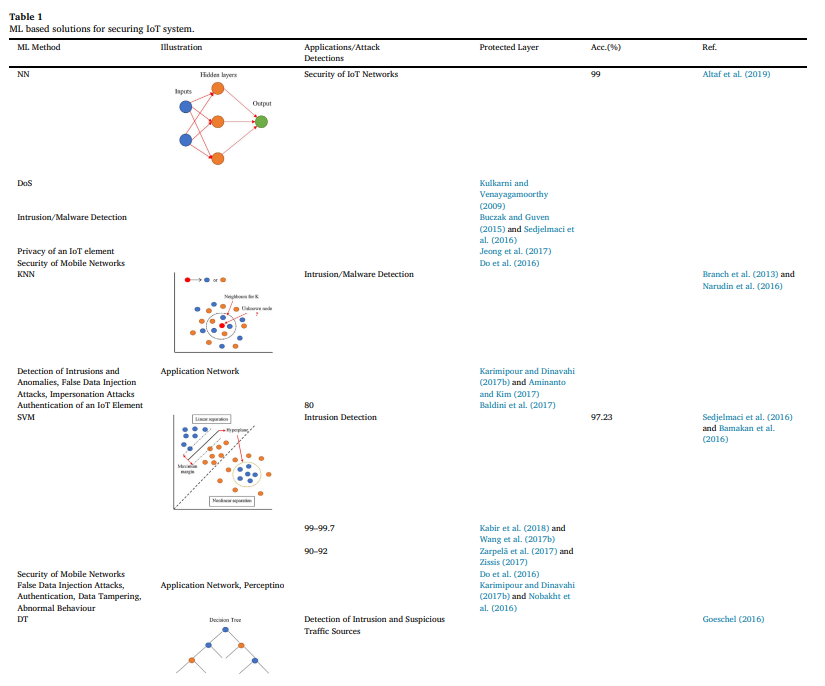
\includegraphics[width=0.9\linewidth]{image.png}
    \caption{Summary of the strengths and weaknesses of the reviewed approaches}
    \label{fig:enter-label}
\end{figure*}

On Fig. 1.\cite{b15} we can see evaluations of security approaches for authentication in IoT system. Based on the table, their strengths and weaknesses mainly depend on environment situations. 
 
\subsection{Safeguarding IoT Devices and Networks}

Safeguarding IoT devices and networks requires a comprehensive approach that includes a variety of security measures, such as:
\begin{itemize}
    \item Securing IoT devices: 
    
    IoT devices should be secured with strong authentication mechanisms, encryption, and security patches.
    \item Segmenting IoT networks: 
    
    IoT networks should be segmented to isolate critical systems from less critical systems.
    \item Monitoring IoT networks:
    
    IoT networks should be monitored for suspicious activity and security threats.
    \item Implementing security policies and procedures: 
    
    Organizations should implement and enforce security policies and procedures to protect their IoT systems.
\end{itemize}


\subsection{Innovations in IoT Security: Blockchain and Machine Learning Applications
}
Blockchain and machine learning are two emerging technologies that have the potential to revolutionize IoT security.

Blockchain is a distributed ledger technology that can be used to create secure and tamper-proof records. This makes it ideal for a variety of IoT security applications, such as device authentication, data privacy, and auditability.

Machine learning can be used to develop intelligent security solutions that can detect and respond to security threats in real time. This is particularly important for IoT systems, which are often under constant attack.

\begin{figure*}
    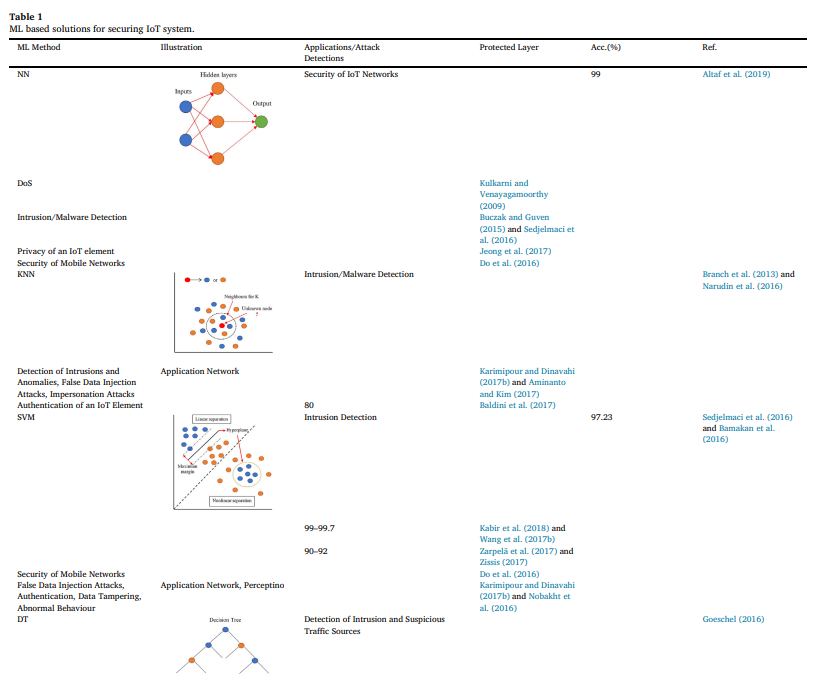
\includegraphics[width=0.9\linewidth]{image1.png}
    \caption{ML based solutions for security}
    %\label{fig:enter-label}
\end{figure*}
On Fig. 2.\cite{b16} we can see best ML based solutions for security. These supervised learning soultions (K-NN, RF, Q-learning, Dyna-Q) are already widely used to secure IoT systems from malware, web and application attacks today.

\subsection{Establishing a Resilient and Secure IoT Infrastructure} 

Establishing a resilient and secure IoT infrastructure requires a holistic approach that combines innovative technologies and solutions with sound security practices.

Some of the key elements of a resilient and secure IoT infrastructure include:

\begin{itemize}
    \item Risk assessment and management:
    
    Organizations should conduct regular risk assessments to identify and mitigate security risks to their IoT systems.
    \item Security by design:
    
    IoT devices and networks should be designed with security in mind.
    \item Zero trust security: 
    
    Organizations should implement a zero
\end{itemize}


\section{Authentication and Data Privacy in IoT Systems}
\subsection{Authentication}

Authentication is the process of verifying the identity of a user or device. In the context of the Internet of Things (IoT), authentication is essential for ensuring that only authorized users and devices can access IoT systems and data. This is crucial for preventing unauthorized access to sensitive data, controlling access to IoT devices and services, and protecting against cyberattacks.

There are several key aspects of authentication in IoT systems:

\begin{itemize}
    \item Entity Identification: Each device, user, or application involved in the IoT network must have a unique identifier, such as a username, device ID, or serial number.
    \item Credential Verification: The entity must provide valid credentials, such as a password, digital certificate, or biometric information, to prove its identity.
    \item Access Control: Based on the verified identity, the system enforces access control policies, granting or denying access to specific resources or services.
    \item Mutual Authentication: In some cases, mutual authentication is employed, where both the entity and the system verify each other's identities to ensure secure communication.
    \item Strong Authentication Mechanisms: Strong authentication mechanisms, such as multi-factor authentication (MFA), should be implemented to enhance security and prevent unauthorized access.
    \item Credential Management: Secure credential storage, transmission, and revocation mechanisms are essential to protect against credential theft and compromise.
    \item Identity and Access Management (IAM) Systems: IAM systems can provide centralized management of user identities, access permissions, and authentication protocols for large-scale IoT deployments.
\end{itemize}

\subsection{Data Privacy}

Data privacy is the right of an individual to control their personal data. In the context of the IoT, data privacy is critical because IoT devices often collect a large amount of personal data, such as location data, health data, and usage patterns. This data can be used to track the user's movements, monitor their health, and even target them with advertising.

There are several key principles for protecting data privacy in IoT systems:

\begin{itemize}
    \item Data Minimization: Only collect the data that is necessary for the specific purpose for which it is being collected. Avoid collecting excessive or irrelevant data that could compromise user privacy.
    \item Data Encryption: Encrypt sensitive data at rest and in transit to protect it from unauthorized access or interception. Encryption algorithms should be strong and regularly updated to maintain security.
    \item Data Anonymization: Anonymize or pseudonymize personal data when appropriate to remove direct identification with individuals. This can help protect privacy while still allowing for data analysis or personalization.
    \item Data Access Control: Implement access control mechanisms to restrict access to personal data to authorized personnel or applications. Limit data sharing and ensure proper consent procedures.
    \item Data Security Awareness: Educate employees and users about data privacy risks and best practices. Encourage responsible data handling and reporting of any potential privacy breaches.
    \item Data Breach Response: Establish clear procedures for responding to data breaches, including notifying affected individuals, containing the breach, and implementing corrective measures.
    \item Compliance with Privacy Regulations: Adhere to relevant privacy regulations, such as the General Data Protection Regulation (GDPR) or the California Consumer Privacy Act (CCPA), which govern the collection, use, and disclosure of personal data.
\end{itemize}

\subsection{Challenges}

There are a number of challenges that need to be addressed in order to ensure authentication and data privacy in IoT systems:

\begin{itemize}
    \item Heterogeneity of IoT Devices: The vast array of IoT devices with varying capabilities and security implementations makes it difficult to implement uniform security standards.
    \item Lack of Standardization: The absence of standardized security protocols for IoT devices hinders the development of interoperable and secure IoT ecosystems.
    \item Scalability: Managing authentication and data privacy for millions of IoT devices across a distributed network poses significant scalability challenges.
    \item Resource Constraints: Resource-constrained IoT devices may struggle to implement complex authentication and encryption algorithms, requiring alternative approaches to security.
    \item Evolving Security Threats: Continuously evolving cyber threats and attack vectors demand constant vigilance and adaptation of security measures in IoT systems.
    \item Balancing Security and Usability: Implementing robust security measures should not compromise user experience or hinder the functionality of IoT devices.
\end{itemize}

\subsection{Conclusion}

Authentication and data privacy are fundamental aspects of securing IoT systems and protecting user information. By implementing appropriate security measures, organizations can safeguard their IoT deployments, maintain user trust, and comply with data privacy regulations. Addressing the challenges mentioned above is crucial for building a secure and privacy-respecting IoT ecosystem.

\begin{table}[h]
\centering
\small
\caption{Authentication Methods}
\begin{tabular}{|p{0.75cm}|p{2.25cm}|p{1.75cm}|p{2.25cm}|}
\hline
\textbf{Method} & \textbf{Description} & \textbf{Advantages} & \textbf{Disadvantages} \\
\hline
Pass-word-based & Users enter a username and password to verify their identity. & Simple to implement and use. & Vulnerable to password attacks, such as brute-force attacks and phishing. \\
\hline
Biomet
ric & Users provide a physical characteristic, such as their fingerprint or facial features, for identification. & Strong security and resistance to unauthorized access. & Requires specialized hardware and may have privacy concerns. \\
\hline
Token-based & Users possess a physical token, such as a smart card or USB key, to authenticate. & Can provide additional security beyond passwords. & May be lost or stolen, and physical access to the token is required. \\
\hline
Certifi-cate-based & Devices or users exchange digital certificates to establish trust and verify identities. & Strong security and support for mutual authentication. & Requires infrastructure for certificate issuance and management. \\
\hline
\end{tabular}
\end{table}





\section{Safeguarding IoT Devices and Networks}

Safeguarding Internet of Things devices and networks is of paramount importance in today's interconnected world. IoT devices, which include everything from smart thermostats and security cameras to industrial sensors and medical equipment, have become ubiquitous, providing convenience and efficiency but also introducing security vulnerabilities. To protect these devices and the networks they connect to, a comprehensive approach is necessary.

\begin{figure}
    \centering
    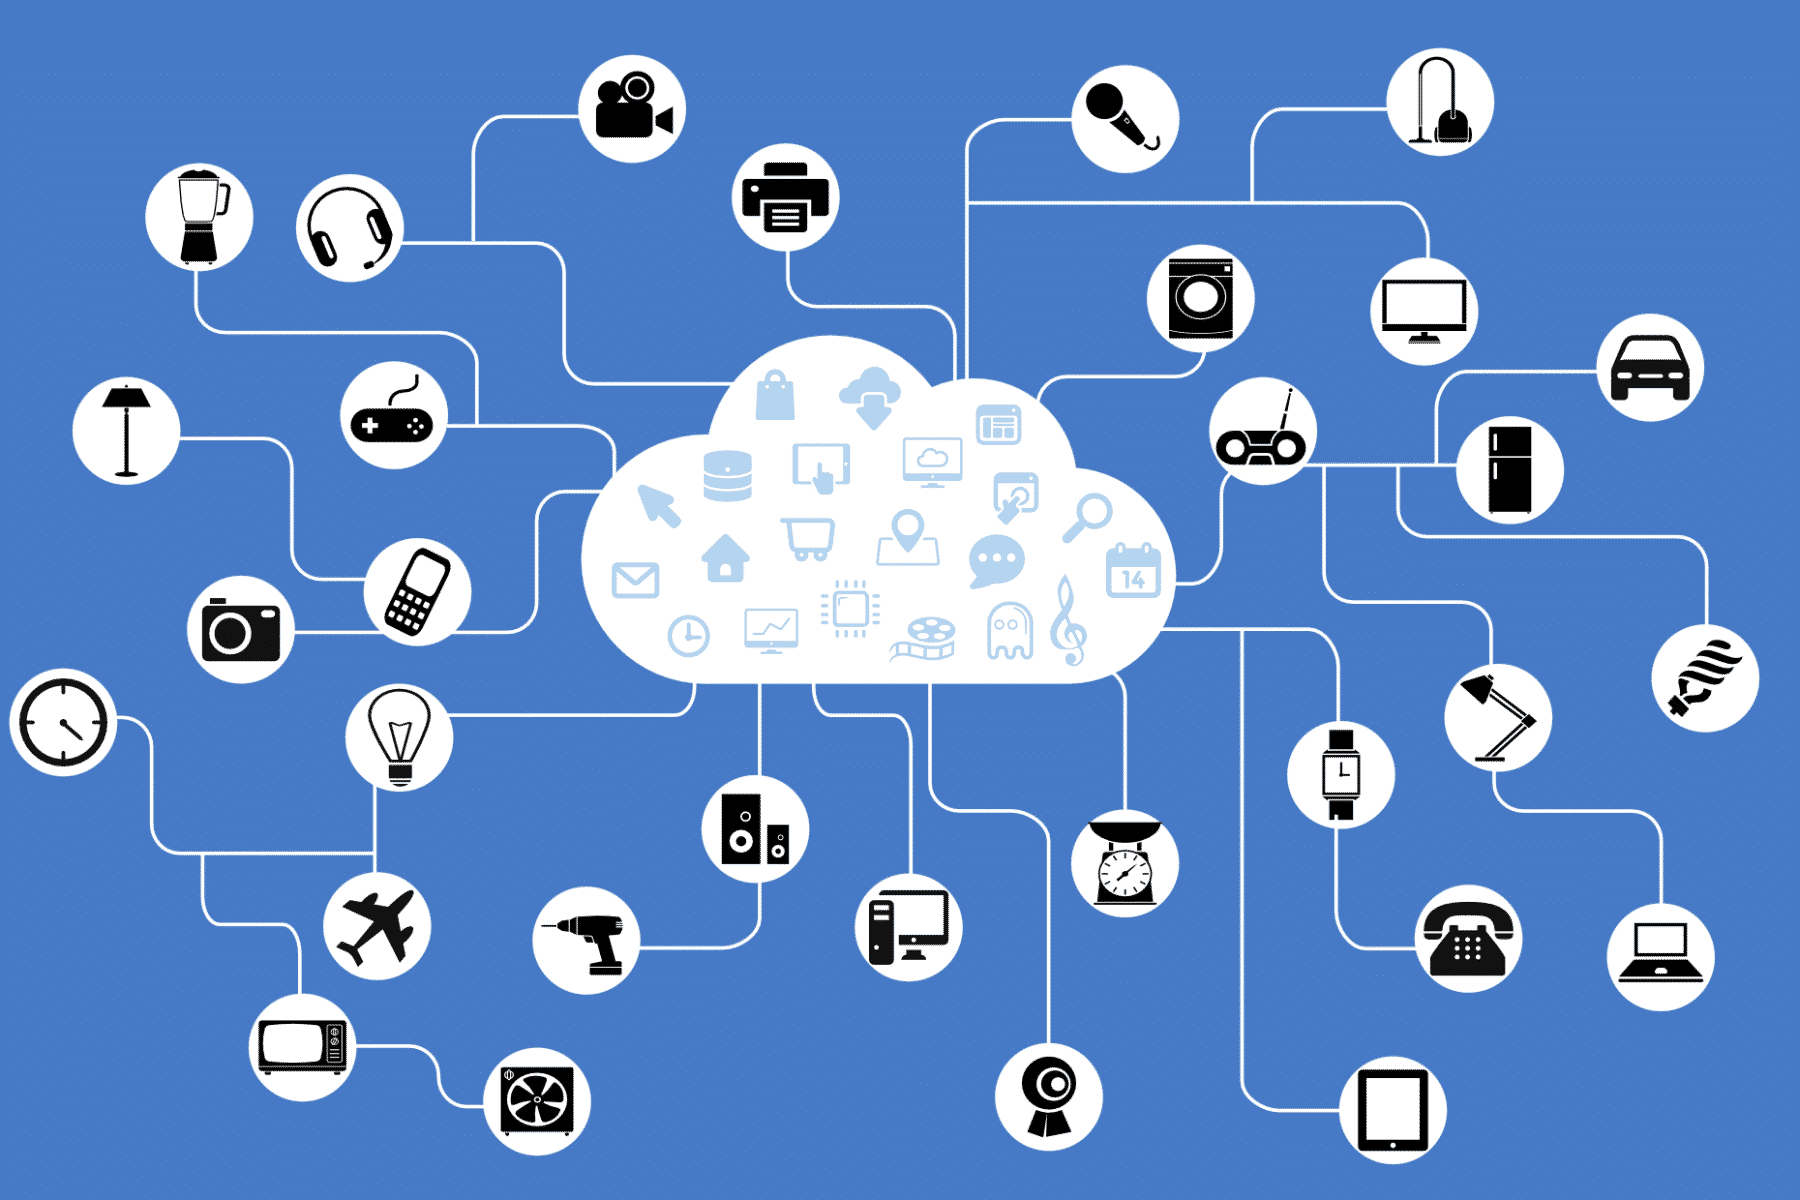
\includegraphics[width=1.1\linewidth]{asset-25.png}
    \caption{Safeguarding electronic devices from cyber threats}
    \label{fig:enter-label}
\end{figure}

Here are some essential measures and best practices for safeguarding IoT devices and networks:

\begin{itemize}
    \item Secure Authentication and Authorization:
    
Use strong, unique passwords for each IoT device and network component.
Implement multi-factor authentication to add an extra layer of security.
Employ strong encryption protocols to protect authentication credentials during transmission.
    \item Regular Software Updates and Patch Management:

Keep IoT devices and their firmware up to date with the latest security patches and updates.
Enable automatic updates whenever possible to ensure ongoing protection against known vulnerabilities.
    \item Network Segmentation:

Segment your IoT devices into isolated networks or VLANs, separating them from critical systems and data.
Implement strict access controls and firewall rules to limit communication between IoT devices and other network segments.
    \item Network Monitoring and Intrusion Detection:

Deploy intrusion detection systems and intrusion prevention systems to detect and respond to suspicious activity.
Continuously monitor network traffic and device behavior to identify anomalies and potential security breaches.
    \item Data Encryption:

Encrypt data both in transit and at rest to protect sensitive information from interception and unauthorized access.
Use strong encryption algorithms and protocols, such as SSL/TLS, to secure data communication.
\end{itemize}

\begin{figure}
    \centering
    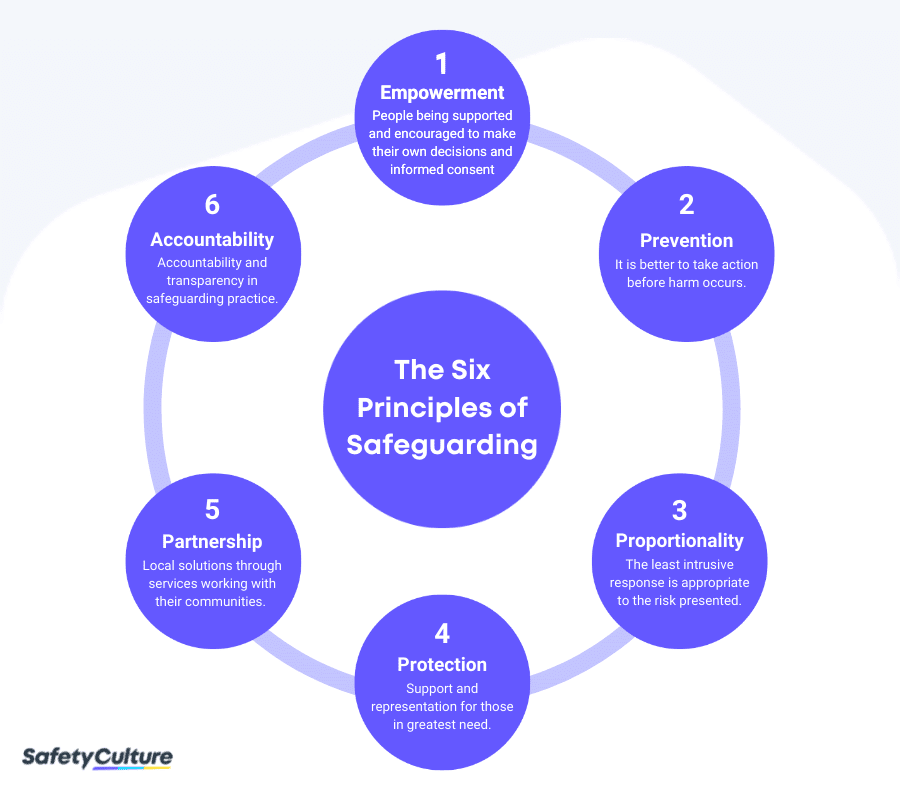
\includegraphics[width=1\linewidth]{6-Principles-of-Safeguarding.jpg}
    
\end{figure}
\section{Innovations in IoT Security: Blockchain and Machine Learning Applications}

Innovations in IoT security have become increasingly important as the number of Internet of Things devices continues to grow. Two key technologies that are making a significant impact in enhancing IoT security are blockchain and machine learning. These innovations offer advanced solutions to tackle the challenges of securing IoT ecosystems.

\subsection{Blockchain in IoT Security}
Blockchain technology, often associated with cryptocurrencies like Bitcoin, provides a distributed and immutable ledger that is proving to be a game-changer in IoT security. Here are some key ways in which blockchain is transforming IoT security:

\begin{itemize}
    \item Immutable Data Integrity: 
    
    Blockchain records transactions in a tamper-proof and unchangeable ledger. In IoT, this means that data generated by devices can be securely stored and verified without the risk of unauthorized alterations.
    \item Decentralized Trust:
    
    Blockchain eliminates the need for a central authority, reducing the risk of single points of failure. This is crucial for IoT networks that are often decentralized by design.
    \item Device Authentication: 
    
    Blockchain can be used to securely authenticate IoT devices. Each device can have a unique identity stored on the blockchain, which is used for secure communication and access control.
    \item Secure Data Sharing:
    
    Blockchain enables secure data sharing between devices and parties in a network, enhancing the privacy and security of IoT data exchanges.
    \item Smart Contracts:
    
    Smart contracts on blockchain platforms like Ethereum can automate security processes, such as access control, without human intervention, improving the efficiency of security protocols.
\end{itemize}


\begin{figure}
    \centering
    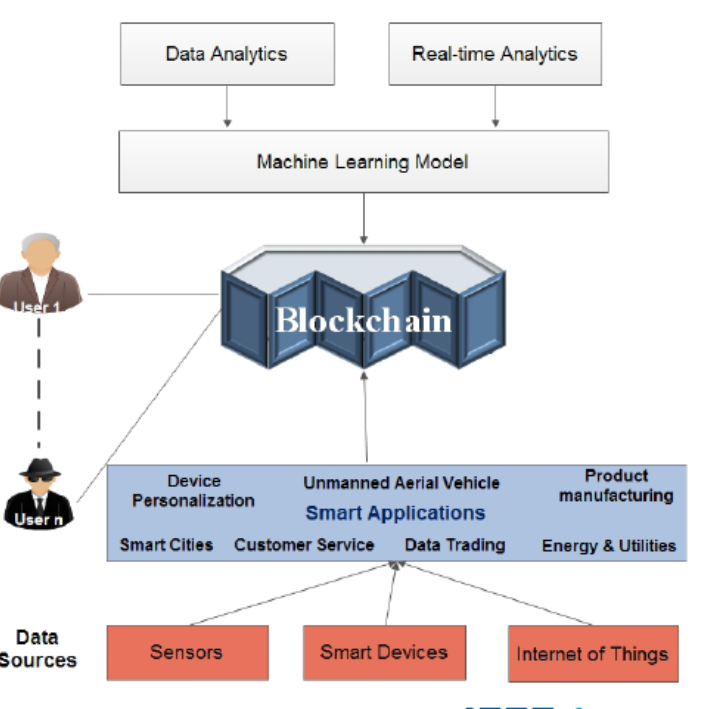
\includegraphics[width=1\linewidth]{image-84.png}
    \caption{The way how ML can be used with Blockchain}
    \label{fig:enter-label}
\end{figure}

\subsection{Machine Learning Applications in IoT Security} 
Machine learning is a subset of artificial intelligence that is being used to enhance IoT security in several ways:

\begin{itemize}
    \item Anomaly Detection: 
    
    Machine learning algorithms can analyze the behavior of IoT devices and detect anomalies in real-time. If a device starts behaving unusually, it can trigger an alert, helping to identify potential security threats.
    \item Predictive Analytics:
    
    Machine learning can predict security threats based on historical data. By analyzing patterns and trends, it can anticipate and mitigate potential attacks before they occur.
    \item Behavioral Profiling:
    
    Machine learning can create behavioral profiles for IoT devices, enabling security systems to detect when a device is behaving abnormally or being controlled by an unauthorized entity.
    \item Network Traffic Analysis: 
    
    Machine learning can scrutinize network traffic for unusual patterns, helping to identify and respond to suspicious activities or attacks.
    \item Improving Authentication:
    
    Machine learning can enhance authentication methods, including biometric authentication for users interacting with IoT devices, making it more difficult for malicious actors to gain unauthorized access.
    \item Vulnerability Management: 
    
    Machine learning can assist in identifying vulnerabilities in IoT devices and applications, helping organizations to patch or mitigate these vulnerabilities proactively.

\end{itemize}

The integration of blockchain and machine learning can provide even more robust security for IoT ecosystems. For example, blockchain can be used to securely store machine learning models and training data, while machine learning can continuously analyze the blockchain for suspicious activity.

\section{Establishing a Resilient and Secure IoT Infrastructure}

\label{sec:iot-security}

The Internet of Things (IoT) has transformed our world, seamlessly connecting devices and enabling a vast network of interconnected systems. While IoT offers immense benefits, it also introduces unique security challenges, demanding a robust approach to safeguarding the connected ecosystem. Establishing a resilient and secure IoT infrastructure is paramount for organizations seeking to harness the full potential of IoT while protecting their valuable assets and data.

\subsection{Key Considerations for Building a Resilient and Secure IoT Infrastructure}

\subsubsection{Device Identity and Access Management}

The foundation of a secure IoT infrastructure lies in establishing strong authentication mechanisms for device identification and authorization. Employing unique device identifiers and implementing role-based access control (RBAC) ensures that only authorized devices and users can access sensitive data and resources. Regular firmware updates for devices are crucial to address vulnerabilities and maintain a secure posture.

\subsubsection{Network Security}

Network security is essential for protecting IoT devices from unauthorized access and malicious attacks. Segmenting IoT networks into isolated zones minimizes the attack surface and prevents lateral movement of threats. Deploying firewalls and intrusion detection/prevention systems (IDS/IPS) provides a layered approach to network defense, monitoring network traffic for suspicious activity and preventing unauthorized access. Data encryption in transit and at rest safeguards sensitive information from interception and unauthorized access.

\subsubsection{Data Security}

Data security is paramount in the IoT ecosystem, where vast amounts of data are collected, processed, and transmitted. Employing strong encryption techniques, such as AES or RSA, protects sensitive data at rest and in transit, preventing unauthorized access and breaches. Data masking and anonymization techniques safeguard privacy by obscuring sensitive information while preserving its utility for analysis. Regularly reviewing and updating data security policies and procedures ensures that data handling practices align with evolving threats and industry standards.

\subsubsection{Vulnerability Management}

A comprehensive vulnerability management program is essential for identifying, assessing, and prioritizing vulnerabilities across the IoT infrastructure. Implementing automated vulnerability scanning tools and employing expert security analysts help uncover potential weaknesses in devices, software, and network configurations. Prioritizing vulnerabilities based on their severity and potential impact enables organizations to focus their remediation efforts on the most critical threats.

\subsubsection{Security Monitoring and Incident Response}

Continuous monitoring of IoT networks and devices is crucial for detecting and responding to security incidents promptly. Implementing security information and event management (SIEM) tools provides centralized visibility into network activity, allowing for real-time threat detection and analysis. Establishing a robust incident response plan ensures that organizations can effectively handle security breaches, minimizing damage and restoring normal operations quickly. Regular penetration testing simulates real-world attacks, identifying potential security gaps and vulnerabilities before they can be exploited by malicious actors.

\subsubsection{Secure Software Development Practices}

Integrating security into the software development lifecycle (SDLC) is essential for building secure IoT applications. DevSecOps practices, which combine security expertise with development processes, ensure that security considerations are embedded throughout the software development process. Employing static and dynamic code analysis tools helps identify and fix vulnerabilities early in the development cycle, preventing them from being introduced into production environments. Conducting thorough security testing before deploying IoT applications ensures that they meet security requirements and can withstand potential attacks.

\subsubsection{Physical Security}

Physical security measures are crucial for protecting IoT devices from unauthorized access, tampering, or theft. Implementing physical barriers, access control systems, and surveillance cameras safeguards IoT devices from physical intrusion. Securely storing and disposing of IoT devices at the end of their lifecycle prevents data leaks or unauthorized access to sensitive information. Educating employees on physical security best practices minimizes human error and promotes a culture of security awareness.

\subsubsection{User Education and Awareness}

User education and awareness are critical components of a comprehensive IoT security strategy. Providing regular security training to employees on IoT security risks and best practices ensures that they understand their role in protecting the organization's assets. Encouraging strong password practices and implementing multi-factor authentication for user accounts adds an extra layer of protection against unauthorized access. Promoting awareness of phishing attacks and social engineering tactics helps employees identify and avoid these common attack vectors, preventing credential theft and data breaches.

\subsection{Conclusion}

Establishing a resilient and secure IoT infrastructure requires a holistic approach that encompasses device security, network security, data security, vulnerability management, security monitoring, secure software development practices, physical security, and user education. By implementing these strategies, organizations can effectively protect their IoT deployments, mitigate potential security risks, and reap the full benefits of the connected world while maintaining a high level of security and compliance.


\section{Conclusion}
To conclude, The rapid integration of the Internet of Things (IoT) has brought about unprecedented innovation and connectivity, transforming various industries and reshaping daily life experiences. However, this proliferation has also unveiled a multitude of security challenges that threaten the integrity and reliability of the IoT ecosystem. With the potential for unauthorized access, data breaches, and the vulnerability of interconnected devices, ensuring robust security measures is imperative for fostering a safe and trustworthy environment for the continued growth of IoT technologies.

The complexities of the IoT landscape, coupled with the significant volume of personal data collected by these devices, underscore the critical need for prioritizing data privacy. With data serving as a potent tool for tracking, monitoring, and targeting, organizations must adhere to key principles, including data minimization, encryption, anonymization, access control, and stringent compliance with privacy regulations. By mitigating the challenges posed by the heterogeneity of IoT devices, the lack of standardization, scalability issues, resource constraints, evolving security threats, and the delicate balance between security and usability, the foundation can be laid for a more secure and resilient IoT ecosystem.

Safeguarding IoT devices and networks necessitates a comprehensive approach, integrating secure authentication and authorization, network segmentation, continuous monitoring, and data encryption. The adoption of intrusion detection systems, firewalls, and strict security policies can significantly reduce vulnerabilities and fortify the network against potential cyber threats. Moreover, innovations in IoT security, particularly the integration of blockchain and machine learning applications, have proven instrumental in enhancing data integrity, decentralizing trust, ensuring device authentication, and fostering secure data sharing. Leveraging these technologies in conjunction with each other not only strengthens the overall security posture but also offers sophisticated solutions for threat detection and analysis.

Establishing a resilient and secure IoT infrastructure demands a strategic blend of device and network security measures, data protection protocols, vulnerability management, robust security monitoring, secure software development practices, physical security implementation, and comprehensive user education. By prioritizing these considerations, organizations can proactively safeguard their IoT deployments, preempt potential security risks, and foster a culture of security awareness within their workforce. As the IoT landscape continues to evolve, it is imperative for stakeholders to remain vigilant, adaptive, and informed about emerging security paradigms, enabling them to navigate the complexities of the interconnected world while upholding the highest standards of security and compliance. By adhering to these best practices and embracing a holistic approach to IoT security, organizations can effectively harness the transformative potential of IoT while ensuring the protection and privacy of sensitive data and assets.


\begin{thebibliography}{00}

\bibitem{b1} Mazhelis, O., Luoma, E., \& Warma, H. (2012). Defining an Internet-of-Things Ecosystem. Lecture Notes in Computer Science, 1–14. doi:10.1007/978-3-642-32686-8_1  https://sci-hub.se/https://link.springer.com/chapter/10.1007/978-3-642-32686-8_1

\bibitem{b2} Keoh, S. L., Kumar, S. S., \& Tschofenig, H. (2014). Securing the internet of things: A standardization perspective. IEEE Internet of things Journal, 1(3), 265-275. https://sci-hub.se/10.1109/JIOT.2014.2323395

\bibitem{b3} Ravikumar, K. C., Chiranjeevi, P., Devarajan, N. M., Kaur, C., \& Taloba, A. I. (2022). Challenges in internet of things towards the security using deep learning techniques. Measurement: Sensors, 24, 100473. 
https://www.sciencedirect.com/science/article/pii/S2665917422001076
\bibitem{b4} M. A. Al-Garadi, A. Mohamed, A. K. Al-Ali, X. Du, I. Ali and M. Guizani, "A Survey of Machine and Deep Learning Methods for Internet of Things (IoT) Security," in IEEE Communications Surveys \& Tutorials, vol. 22, no. 3, pp. 1646-1685, thirdquarter 2020, doi: 10.1109/COMST.2020.2988293. https://sci-hub.se/10.1109/COMST.2020.2988293

\bibitem{b5}M. Moh and R. Raju, "Machine Learning Techniques for Security of Internet of Things (IoT) and Fog Computing Systems," 2018 International Conference on High Performance Computing \& Simulation (HPCS), Orleans, France, 2018, pp. 709-715, doi: 10.1109/HPCS.2018.00116. https://sci-hub.se/10.1109/HPCS.2018.00116

\bibitem{b6}Noor, M. binti M.,\& Hassan, W. H. (2018). Current research on Internet of Things (IoT) security: A survey. Computer Networks.doi:10.1016/j.comnet.2018.11.025 https://www.sciencedirect.com/science/article/abs/pii/S1389128618307035

\bibitem{b7}Samaila, M. G., Neto, M., Fernandes, D. A. B., Freire, M. M., \& Inácio, P. R. M. (2018). Challenges of securing Internet of Things devices: A survey. Security and Privacy, 1(2), e20. doi:10.1002/spy2.20 https://onlinelibrary.wiley.com/doi/full/10.1002/spy2.20

\bibitem{b8}Gan, G., Lu, Z., \& Jiang, J. (2011). Internet of Things Security Analysis. 2011 International Conference on Internet Technology and Applications. doi:10.1109/itap.2011.6006307 

https://sci-hub.se/10.1109/ITAP.2011.6006307
\bibitem{b9}Alaba, F. A., Othman, M., Hashem, I. A. T., \& Alotaibi, F. (2017). Internet of Things security: A survey. Journal of Network and Computer Applications, 88, 10-28. 

https://www.sciencedirect.com/science/article/abs/pii/S1084804517301455
\bibitem{b10}Guarda, T., Leon, M., Augusto, M. F., Haz, L., de la Cruz, M., Orozco, W., \& Alvarez, J. (2017). Internet of Things challenges. 2017 12th Iberian Conference on Information Systems and Technologies (CISTI). doi:10.23919/cisti.2017.7975936 https://sci-hub.se/10.23919/CISTI.2017.7975936

\bibitem{b11}Grammatikis, P. I. R., Sarigiannidis, P. G., \& Moscholios, I. D. (2019). Securing the Internet of Things: Challenges, threats and solutions. Internet of Things, 5, 41-70. 

https://www.sciencedirect.com/science/article/abs/pii/S2542660518301161
\bibitem{b12}Sisinni, E., Saifullah, A., Han, S., Jennehag, U., \& Gidlund, M. (2018). Industrial Internet of Things: Challenges, Opportunities, and Directions. IEEE Transactions on Industrial Informatics, 1–1. doi:10.1109/tii.2018.2852491 https://sci-hub.se/10.1109/TII.2018.2852491

\bibitem{b13} Mukhopadhyay, S. C., \& Suryadevara, N. K. (2014). Internet of Things: Challenges and Opportunities. Smart Sensors, Measurement and Instrumentation, 1–17. doi:10.1007/978-3-319-04223-7_1 https://sci-hub.se/https://link.springer.com/chapter/10.1007/978-3-319-04223-7\_1

\bibitem{b14} Hartmann, M., \& Halecker, B. (2015). Management of innovation in the industrial internet of things. In ISPIM Conference Proceedings (p. 1). The International Society for Professional Innovation Management (ISPIM). https://www.researchgate.net/profile/Bastian-Halecker/publication/277870196_Management_of_Innovation_in_the_Industrial \
_Internet_of_Things/links/5576b9c808ae7521586c49a1/Management-of-Innovation-in-the-Industrial-Internet-of-Things.pdf

\bibitem{b15} Atwady, Y., \& Hammoudeh, M. (2017). A Survey on Authentication Techniques for the Internet of Things. Proceedings of the International Conference on Future Networks and Distributed Systems  - ICFNDS  ’17. doi:10.1145/3102304.3102312 

\bibitem{b16} Tahsien, S. M., Karimipour, H., \& Spachos, P. (2020). Machine learning based solutions for security of Internet of Things (IoT): A survey. Journal of Network and Computer Applications, 102630. doi:10.1016/j.jnca.2020.102630 

\end{thebibliography}

\end{document}
